%%%%%%%%%%%%%%%%%%%%%  kbb talk %%%%%%%%%%%%%%%%%%%%%%%%%%%%%%%
%%%%%%%%%%%%%%%%%%%%%%%%%%%%%%%%%%%%%%%%%%%%%%%%%%%%%%%%%%%%%%%

\documentclass[12pt,fleqn]{seminar}
\input{seminar.bug}
\pagestyle{empty}
\pdfhorigin=1truein
\pdfvorigin=1truein


% packages
\usepackage{ifpdf}
\usepackage{bm}
\usepackage{latexsym}
\usepackage{color}
\usepackage{pstricks}
\usepackage{ulem} %uwave
\usepackage{amsmath}

\usepackage{amssymb}
%\usepackage{float}
\usepackage{bm}
%\usepackage{wasysym}
%\usepackage[landscape]{geometry}
\usepackage{graphicx}
\usepackage{epstopdf}
\graphicspath{{./Figs/}{./}{../}}
\graphicspath{{/Users/danielhurowitz/PROJ/NEG/Figs/}{./}{../}}



% basic	commands I
\newcommand{\mass}{\mathsf{M}} 
\newcommand{\half}{\mbox{\small $\frac{1}{2}$}}
\newcommand{\sinc}{\mbox{sinc}}
\newcommand{\const}{\mbox{const}}
\newcommand{\trc}{\mbox{trace}}
\newcommand{\intt}{\int\!\!\!\!\int }
\newcommand{\ointt}{\int\!\!\!\!\int\!\!\!\!\!\circ\ }
\newcommand{\eexp}{\mbox{e}^}
\newcommand{\bra}{\left\langle}
\newcommand{\ket}{\right\rangle}
\newcommand{\EPS} {\mbox{\LARGE $\epsilon$}}
\newcommand{\ttimes} {\mbox{\tiny \ $^{\times}$ \ }}
\newcommand{\ar}{\mathsf r}
\newcommand{\im}{\mbox{Im}}
\newcommand{\re}{\mbox{Re}}
\newcommand{\bmsf}[1]{\bm{\mathsf{#1}}} 
\newcommand{\pd}[2]{\frac{\partial #1}{\partial #2}}
\newcommand{\bitem}{$\newline \ \ \bullet \ \ $} 
\newcommand{\ola}{\protect\overleftarrow}
\newcommand{\ora}{\protect\overrightarrow}

% basic	commands II
\newcommand{\hide}[1]{}
\newcommand{\tbox}[1]{\mbox{\tiny #1}}
\newcommand{\Cn}[1]{\begin{center}{#1}\end{center}}
\newcommand{\be}{\begin{eqnarray*}}
\newcommand{\ee}{\end{eqnarray*}}
\newcommand{\beq}{\begin{eqnarray*}}
\newcommand{\eeq}{\end{eqnarray*}}

\newcommand{\mpg}[2][0.45\hsize]{\begin{minipage}[b]{#1}{#2}\end{minipage}}
%
\newcommand{\bmp}[1]{\begin{minipage}[t]{#1}\noindent }
\newcommand{\smp}[1]{\end{minipage}\begin{minipage}[t]{#1}\noindent }
\newcommand{\emp}{\end{minipage}}

\newcommand{\amatrix}[1]{\begin{matrix} #1 \end{matrix}} 


% extra commands for colors
\definecolor{blk}{rgb}{0.,0.,0.}
\definecolor{red}{rgb}{1.,0.,0.}
\definecolor{green}{rgb}{0.,0.5,0.}
\definecolor{blue}{rgb}{0.,0.,1.}
\definecolor{bluek}{rgb}{0.,0.,0.5}
\definecolor{orange}{rgb}{1.,0.56.,0}
\newcommand{\cblk}[1]{\textcolor{blk}{#1}}
\newcommand{\cred}[1]{\textcolor{red}{#1}}
\newcommand{\cgreen}[1]{\textcolor{green}{#1}}
\newcommand{\cblue}[1]{\textcolor{blue}{#1}}
\newcommand{\cbluek}[1]{\textcolor{bluek}{#1}}
\newcommand{\corange}[1]{\textcolor{orange}{#1}}


% extra commands for slides

%\newcommand{\Up}[1][0.5]{\vspace{-#1cm}}
%\newcommand{\Dn}[1][0.5]{\vspace{#1cm}}
%\newcommand{\Tl}[1]{\begin{center}{\bf \small \cblue{#1}}\end{center}}

\newcommand{\Up}[1][5]{\vspace{-#1mm}}
\newcommand{\Dn}[1][5]{\vspace{#1mm}}
\newcommand{\Tl}[1]{\begin{center}{\bf \small \cblue{#1}}\end{center}}

\renewcommand{\slideparindent}{0mm}
\setlength{\mathindent}{0cm} 

% \newcommand{\newsld}{\end{slide}\begin{slide}}


\newcommand{\bslA}[1]{
%portrait
\pdfpagewidth=210truemm
\pdfpageheight=297truemm
\pdfhorigin=1truein
\pdfvorigin=1truein
%portrait
\renewcommand{\slidetopmargin}{0mm}
\renewcommand{\slideleftmargin}{-54mm}
\setlength{\slidewidth}{190mm}
\setlength{\slideheight}{277mm}
\begin{slide}
}



\newcommand{\bslB}[1]{
%landscape
\pdfpagewidth=297truemm
\pdfpageheight=210truemm
\pdfhorigin=1truein
\pdfvorigin=1truein
%portrait 
\renewcommand{\slidetopmargin}{0mm}
\renewcommand{\slideleftmargin}{33mm}
\setlength{\slideheight}{190mm}
\setlength{\slidewidth}{150mm} %130
%portrait fonts
\begin{slide}
\ptsize{8}
}



\newcommand{\bslC}[1]{
%landscape
\pdfpagewidth=297truemm
\pdfpageheight=210truemm
\pdfhorigin=1truein
\pdfvorigin=1truein
%landscape
\renewcommand{\slidetopmargin}{0mm}
\renewcommand{\slideleftmargin}{33mm}
\setlength{\slideheight}{190mm}
\setlength{\slidewidth}{277mm}
%portrait fonts
\begin{slide}
\ptsize{8}
}



\newcommand{\bslD}[1]{
%landscape
\pdfpagewidth=297truemm
\pdfpageheight=210truemm
\pdfhorigin=1truein
\pdfvorigin=1truein
%landscape
\renewcommand{\slidetopmargin}{0mm}
\renewcommand{\slideleftmargin}{33mm}
\setlength{\slideheight}{190mm}
\setlength{\slidewidth}{277mm}
%landscape fonts
\begin{slide}
}



\newcommand{\esl}{\end{slide}}


\newcommand{\vbar}{
\begin{picture}(1,1)
\thicklines
\put(0,61){ \ \ \line(0,-1){280} \ \ } 
\end{picture} 
}


%%%%%%%%%%%%%%%%%%%%%%%%%%%%%%%%%%%%%%%%%%%%%%%%%%%%%%%%%%%%%%%%%%%
%%%%%%%%%%%%%%%%%%%%%%%%%%%%%%%%%%%%%%%%%%%%%%%%%%%%%%%%%%%%%%%%%%%


%%%%%%%%%%%%%%%%%%%%%%%%%%%%%%%%%%%%%%%%%%%%%%%%%%%%%%%%%%%%%%%%%%%
%%%%%%%%%%%%%%%%%%%%%%%%%%%%%%%%%%%%%%%%%%%%%%%%%%%%%%%%%%%%%%%%%%%
\begin{document}
%%%%%%%%%%%%%%%%%%%%%%%%%%%%%%%%
\bslD

\Tl{\Large{Percolation, sliding, localization and relaxation in glassy circuits }}


\Cn{\bf Daniel Hurowitz, Doron Cohen,\\ \corange{Ben-Gurion University}}
%
%
%\bmp{0.5\hsize}
%
%
%
%%\Cn{ \includegraphics[ height=4cm]{}}
%
%\smp{0.5\hsize}
%
%\vspace{0.2cm}
%
%
%
%%{\includegraphics[height=3cm]{ResistorsNetworkBath_a}}
%
%\emp
%
%\bmp{\hsize}



\bmp{0.5\hsize}

\Cn{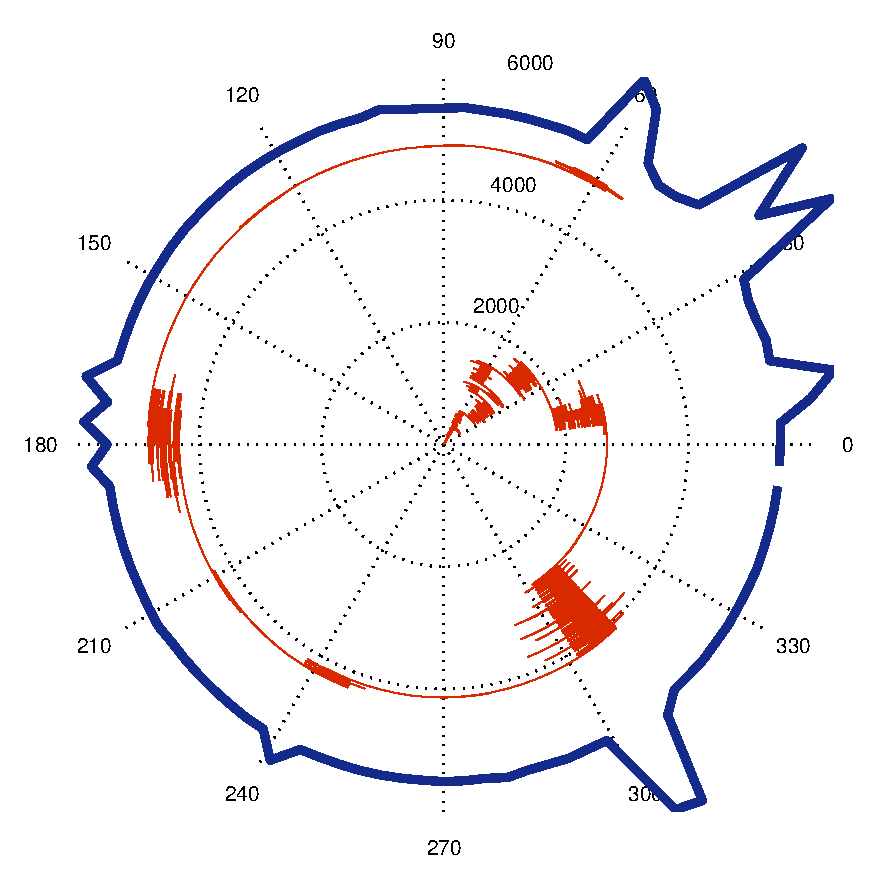
\includegraphics[height=4cm]{/Figs/polar_1_a.eps}}

\smp{0.5\hsize}

\Cn{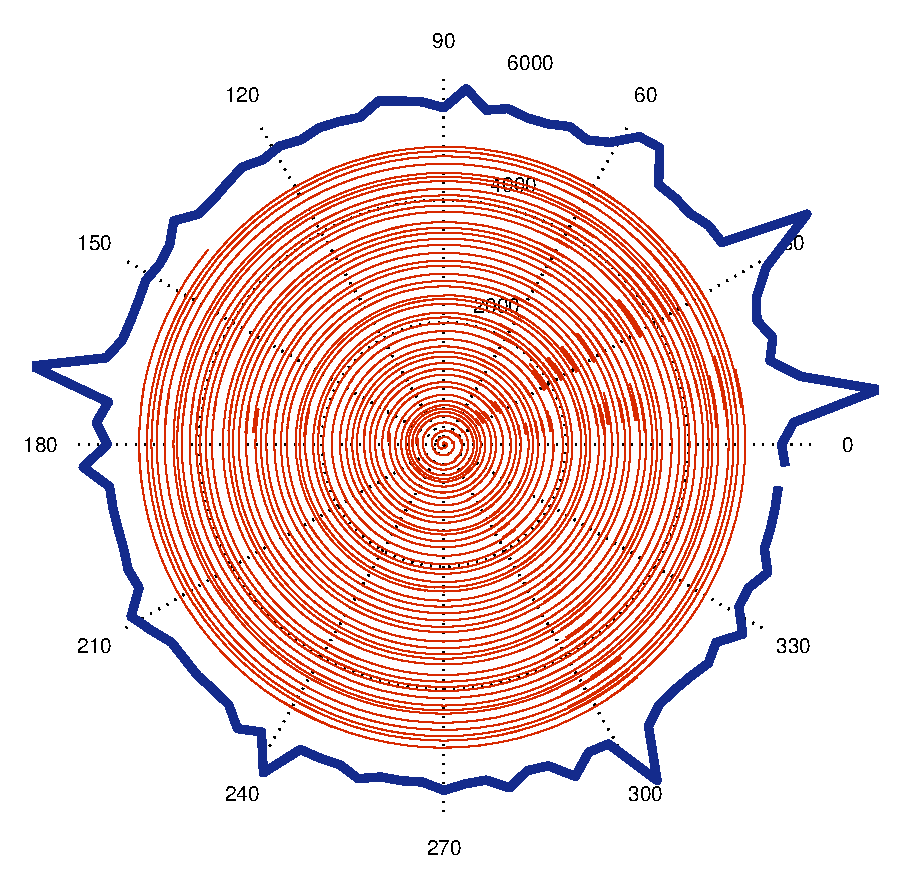
\includegraphics[height=4cm]{/Figs/polar_2_a.eps}}

\emp

\center{{   D. Hurowitz and D. Cohen, \texttt{arXiv} (2014)}}


%\emp

\esl


%%%%%%%%%%%%%%%%%%%%%%%%%%%%%%%%
\bslC

\Tl{\large Brownian motion}


\bmp{0.6\hsize}

\cgreen{{\bf Simple random walk} [Einstein]} 

uniform lattice - all rates are equal $w$,

$D = a^2 w$

\smp{0.4\hsize}


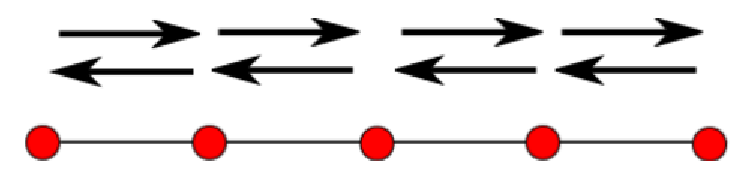
\includegraphics[width=4.5cm]{rw1a}

\emp

\bmp{0.6\hsize}

\cgreen{{\bf Random walk on disordered lattice} [Alexander et. al]} 

Random lattice - random, symmetric transition rates $w_n$

$P(w) \propto w^{\alpha-1}$

 $D = \text{resistor network calculation}$

Percolation related transition to subdiffusion for $\alpha<1$

\smp{0.4\hsize}

\emp

\bmp{0.6\hsize}

\cgreen{{\bf Random walk in random environment} [Sinai, Derrida]} 

Rates allowed to be asymmetric $\displaystyle {\ora{w}_n}/{\ola{w}_n} = e^{\mathcal{E}_n}$

Stochastic field: $\mathcal{E}_n \sim [s-\sigma, \ s+\sigma]$

Sliding transitions for $\displaystyle \left\langle e^{-\mathcal{E} \mu} \right\rangle =1$, defines $s_{\mu}$

$D=0$ for $s<s_{1/2}$

 $v=0$ for $s<s_1$


\smp{0.4\hsize}

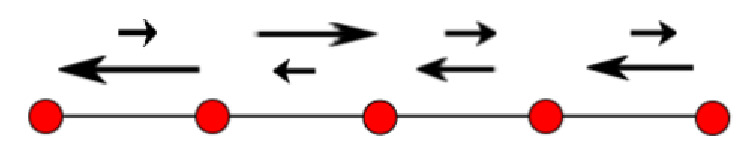
\includegraphics[width=4.5cm]{rw2a}

\emp

\esl

\bslC

\Tl{\large Dynamics}

Stochastic rate equation
%

$\displaystyle
\frac{d\bm{p}}{dt} \ \ = \ \ \bm{W} \bm{p},  \ \ \ \ \ 
\bm{W} \ \ = \ \ \left[\amatrix{
-\gamma_1   & w_{1,2}   & 0         & ... \\ 
w_{2,1}     & -\gamma_2 & w_{2,3}   & ... \\ 
0           & w_{3,2}   & -\gamma_3 & ... \\
...         & ...       & ...       & ...
}\right]
$

with transition rates across $n^{th}$ bond $w_n\eexp{\pm\mathcal{E}_n/2}$

Probability conservation $\sum_n w_{nm} = 0$

Affinity (closed ring) $\displaystyle S_{\circlearrowleft} = \sum_{n=1}^N \log \left(\frac{\ora{w}_n}{\ola{w}_n}\right) \ \ = Ns$

{\bf Relaxation modes of closed ring $\lambda_k$}

How do spectral properties of ${\bm W}$ depend on {$(\alpha,\sigma, s)$?}

\begin{itemize}

\item \cred{\bf What is the threshold bias $s_c$ for complex eigenvalues (delocalization)?}

\item \cred{\bf How is $s_c$ related to the percolation transition? to the sliding transition?}

\item \cred{\bf Implications of conservativity?}

\end{itemize}


\esl


%%%%%%%%%%%%%%%%%%%%%%%%%%%%%%%%%%%%%%%%%%
\bslC

\Tl{\large The spectrum}

\bmp{0.33\hsize}

{
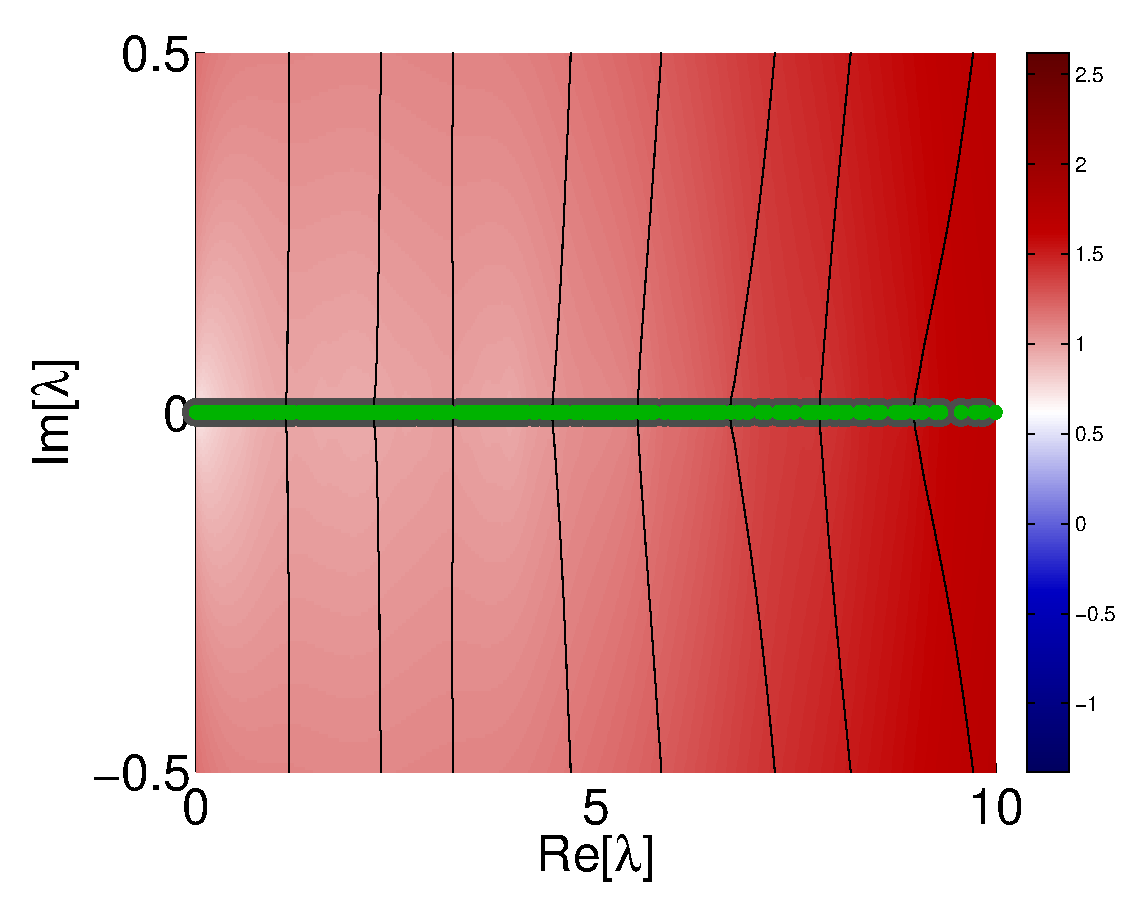
\includegraphics[height=3.5cm]{spectrum_electrostatics1_2}
}

\smp{0.33\hsize}

{
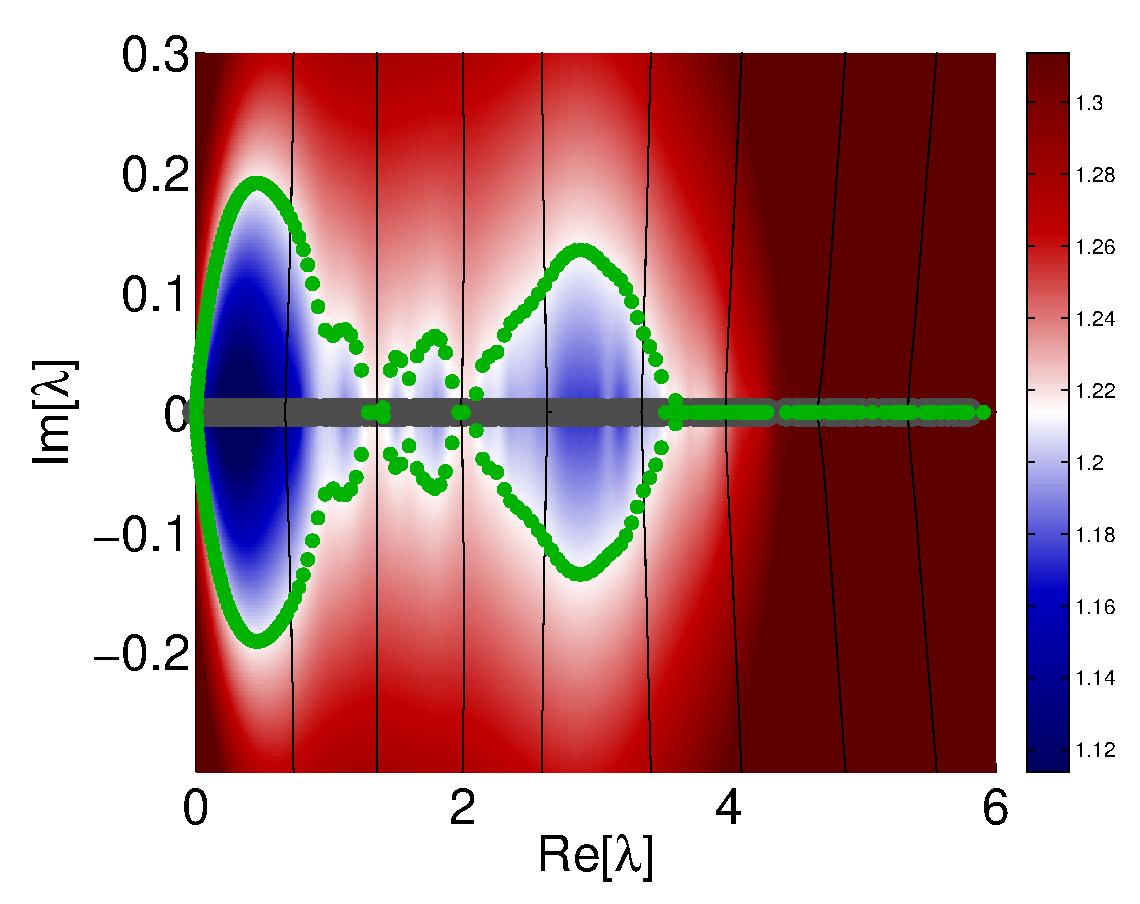
\includegraphics[height=3.5cm]{spectrum_electrostatics1}
}

\smp{0.33\hsize}

{
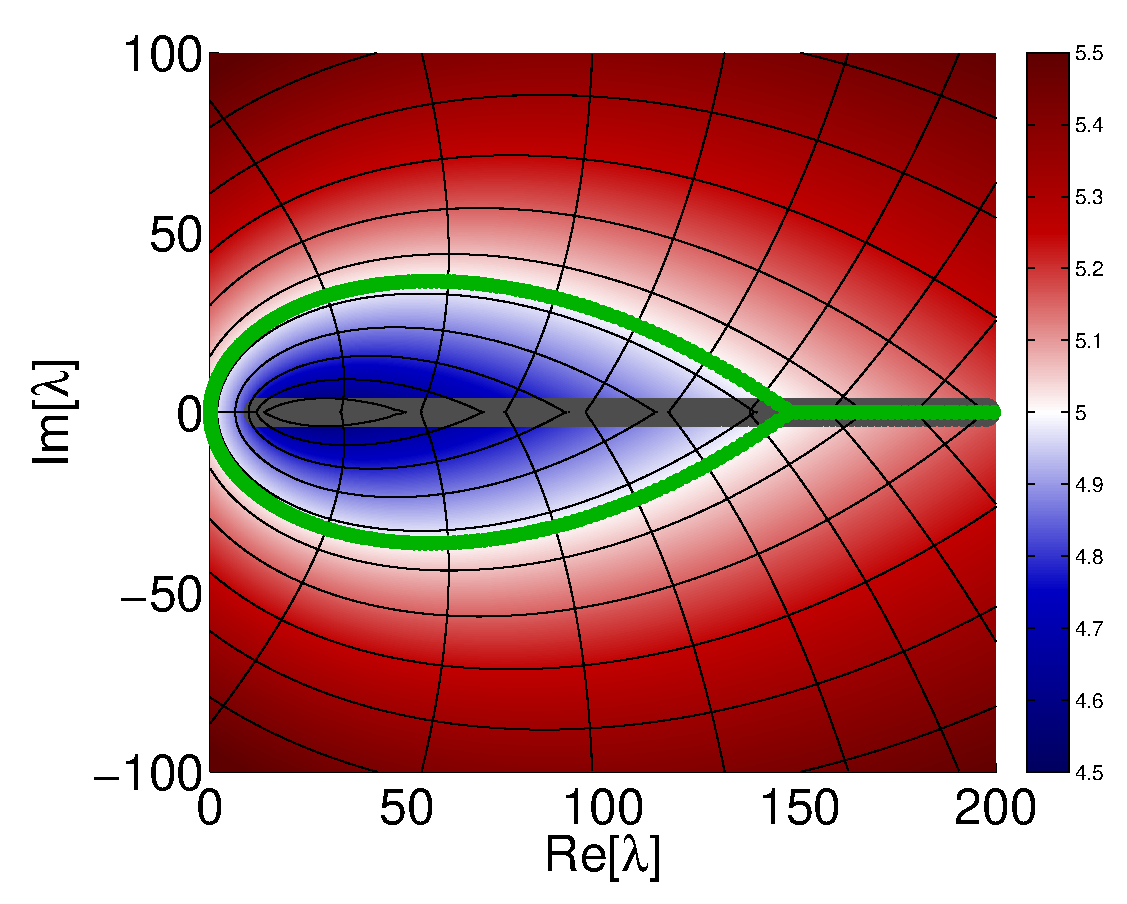
\includegraphics[height=3.5cm]{spectrum_electrostatics2}
}

\emp


\bmp{0.5\hsize}

\begin{itemize}

\item $\lambda_0 = 0$ due to conservativity

\item Complex eigenvalues $\leadsto$ oscillating density

\item Complex bubble at bottom of band

\item Complexity saturation

\end{itemize}

\smp{0.5\hsize}

\hspace{1cm}
%
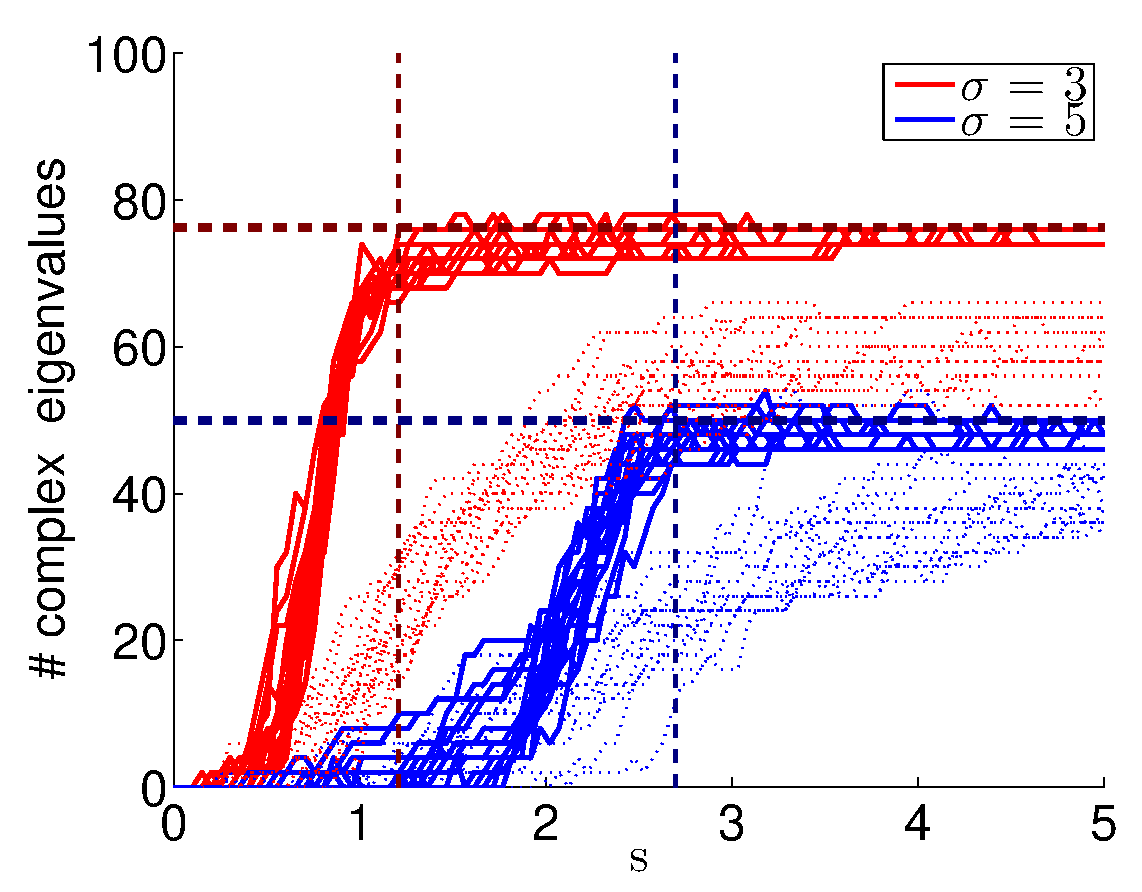
\includegraphics[height=3.5cm]{numComplex_100_alpha_sigma}


\emp

%\Cn{
%
%\cred{\bf What is the threshold bias $s_c$ for complex eigenvalues (delocalization)?}
%
%\cred{\bf How is $s_c$ related to the percolation transition? to the sliding transition?}
%}


\esl
%%%%%%%%%%%%%%%%%%%%%%%%%%%%%%%%%%%%%%%%%%%%%%%%%



%%%%%%%%%%%%%%%%%%%%%%%%%%%%%%%%%%%%%%%%%%

\bslC

\Tl{\large The spectral equation}

Characteristic polynomial $\displaystyle \prod_{k=0}^{N-1} \left(z-\lambda_k\right) \ \ = \ \ 0$

Hatano, Nelson form
$\displaystyle
\prod_{k=0}^{N-1} \left(\frac{z+\epsilon_k(s)}{\overline{w}}\right) \ \ = \ \ 2\left[\cosh\left(\frac{S_{\circlearrowleft}}{2}\right)-1\right]$

\Tl{The associated Hermitian matrix $\bm{H}$}

\cgreen{\bf Open chain}

Gauge away bias 
$
{{\bm{H}} = \eexp{{\bm{U}/2}} \bm{W} \eexp{-{\bm{U}/2}}}
$
 



${\bm H}$ symmetric matrix with real eigenvalues $\epsilon_k (s)$

Density of states 
$
\ \ \rho(\epsilon) \ \propto \ \epsilon^{\mu-1} \ \ \ \ \text{(for small $\epsilon$)}
$

\bmp{0.5\hsize}

{\bf Field disorder }

\vspace{0.2cm}

$\displaystyle
s \ = \ s_{\mu} \ = \ \frac{1}{\mu} \ln\left( \frac{\sinh (\sigma\mu)}{\sigma\mu} \right)
$

\vspace{0.2cm}

For $s>s_{\infty} = \sigma$, gap opens
%
%Velocity vanishes for $s<s_1$
%
%Diffusion vanishes for $s<s_{1/2}$

\smp{0.5\hsize}

{\bf Resistor network disorder}

\vspace{0.2cm}

$\displaystyle
 \mu = \text{min} \left\{ \frac{\alpha}{1+\alpha}, \ \frac{1}{2} \right\}
 $

\vspace{0.2cm}

%For $\alpha > 1$, $\mu=1/2$ (Diffusion)
%
%For $\alpha < 1$, $\mu = \frac{\alpha}{\alpha+1} < 1/2$ (Sub-diffusion)

For large bias,  ${\bm H}$ is trivially localized, $\mu=\alpha$

\emp

\Dn

\cgreen{\bf Closed ring}

Gauge away disorder 
$
{{\bm{\tilde{W}}} = \eexp{{\bm{U}/2}} \bm{W} \eexp{-{\bm{U}/2}}}
$
(cannot gauge away asymmetry)

Associated hermitian matrix ${\bm H}$ with real eigenvalues $\epsilon_k(s)$ by setting $\mathcal{S}_{\circlearrowleft} =0$

%
%

\esl

%%%%%%%%%%%%%%%%%%%%%%%%%%%%%%%%%%%%%%%%%%

\bslC

\Tl{\large Electrostatic picture}

%set $\overline{w}=1, \  z \mapsto -z$

2D Electrostatic potential
%
$\displaystyle \ 
\Psi(z) \ \ = \ \ \sum_k \ln\left(z-\epsilon_k\right) \ \ \equiv \ \ V(x,y)+iA(x,y)
$

The secular equation
%
$\displaystyle
\ \ \ \ \ \ V(x,y)=V(0)=\ln\left[ 2(\cosh(S_{\circlearrowleft}/2)-1)\right]; \ \ \ \ A(x,y)=2\pi*\text{integer} 
$



\Cn{
\cred{\bf Condition for complexity $V(\epsilon) < V(0)$}
}


\cgreen{\bf Continuum approximation}

Density of states $\iff$ charge density $\rho \propto \epsilon^{\mu-1}$

Potential along real axis
%
$\displaystyle
V(\epsilon) \ \ = \ \  \int \ln \left(|\epsilon-x' \right|) \rho(x')dx' \ \ \ \ \text{}
$
%
%Potential at origin
%$\displaystyle
%\ \ \ \ \ \ \ \ V(0) \ \ = \ \ \ln\left[ 2(\cosh(S_{\circlearrowleft}/2)-1)\right]
%$

Derivative at origin
%
$\displaystyle
 \ \ \ \ \ \  V'(\epsilon) \ \ \approx  \ \ \frac{ \epsilon^{\mu-1}}{\epsilon_c^{\mu}} \pi \mu \cot(\pi \mu)
$
, changes sign at $\mu=1/2$



\Cn{
\cred{\bf Condition for complexity $V'(\epsilon) < 0$}
}



\bmp{0.33\hsize}

{
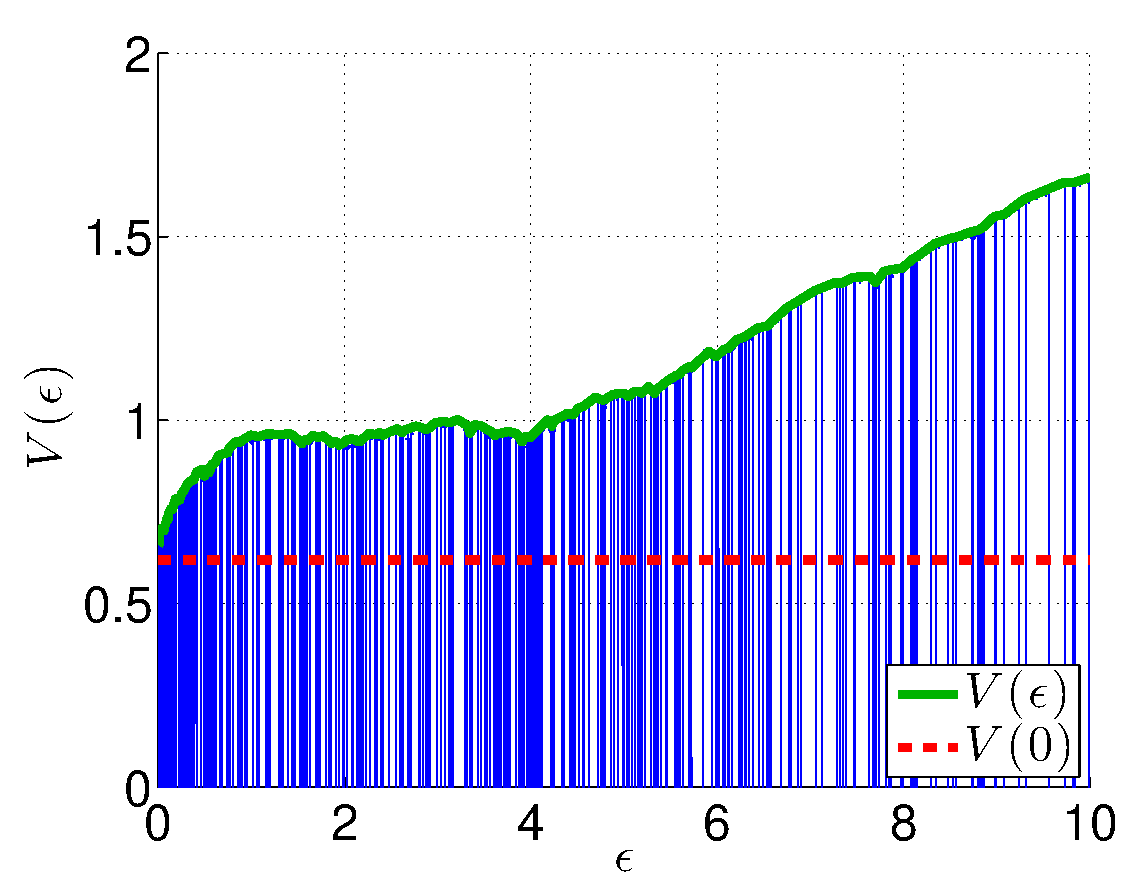
\includegraphics[height=3cm]{V_E_1_2b}

\Cn{$s<s_{1/2}$}

}

\smp{0.33\hsize}

{
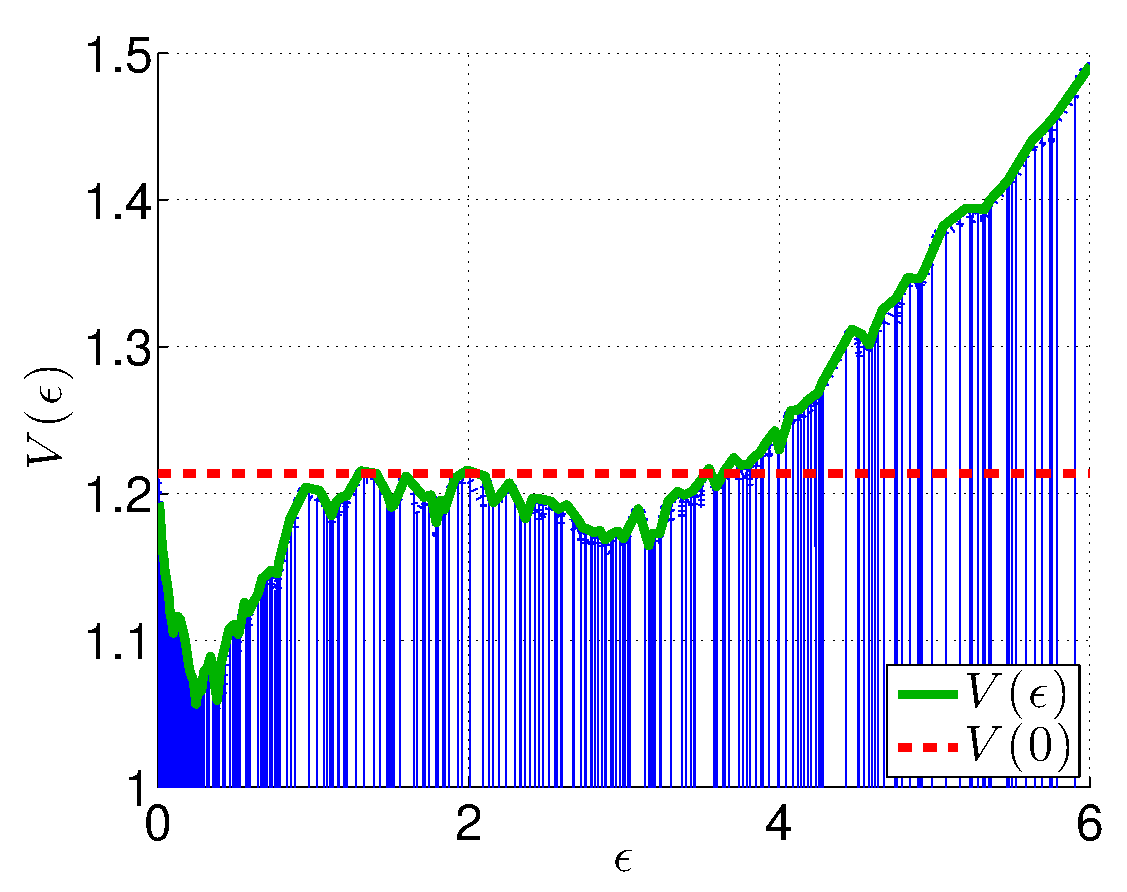
\includegraphics[height=3cm]{V_E_1b}

\Cn{$s>s_{1/2}$}

}

\smp{0.33\hsize}

{
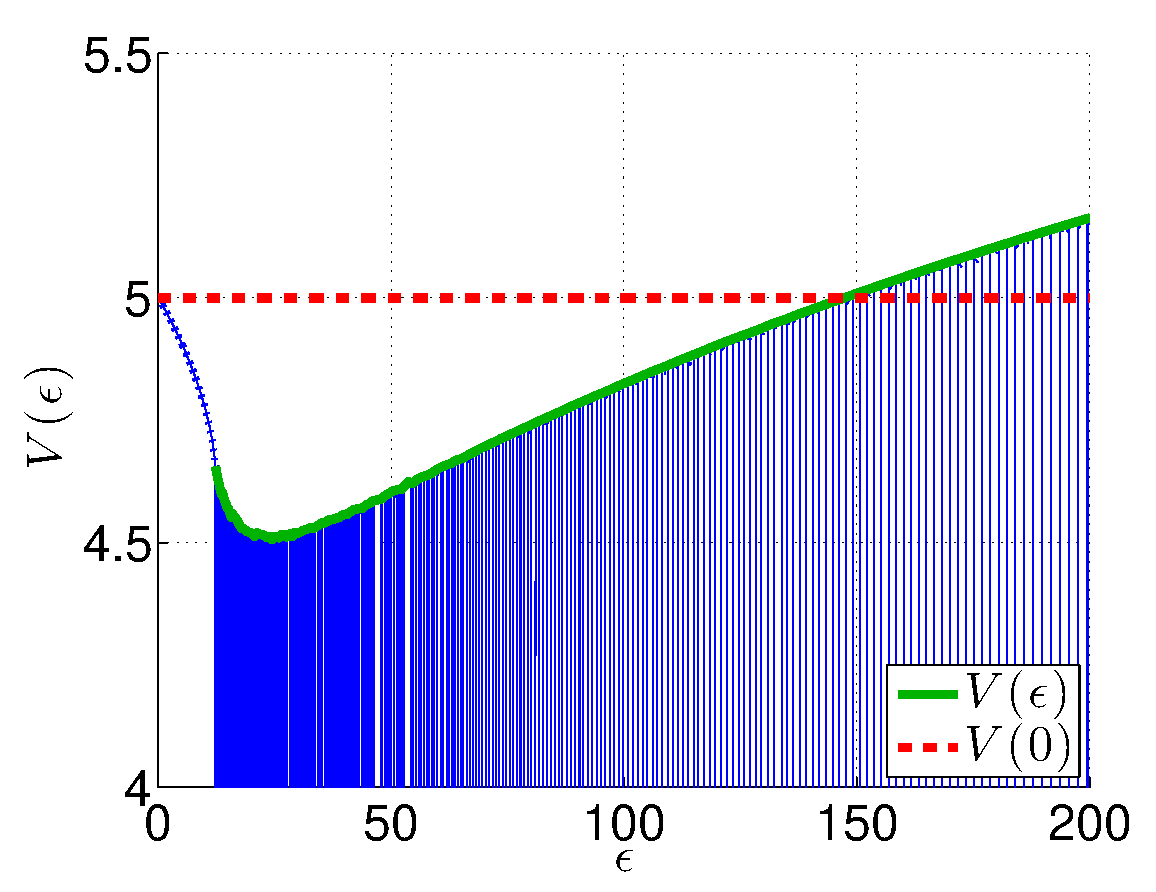
\includegraphics[height=3cm]{V_E_2b}

\Cn{$s>s_{\infty}$}

}



\emp

\esl

\bslC

\Tl{Examples}

{\bf Stochastic field, $\mu=\mu_s(\sigma)$}

$\displaystyle s_c = s_{1/2} < s_1$



\bmp{0.6\hsize}

{\bf Resistor network, $\mu=\mu_{\alpha}$}

\Dn

$\displaystyle
\left\{ 
\begin{matrix}
s=0 & \text{resistor network} & \rightarrow & \mu &=& \frac{\alpha}{1+\alpha} \\
\text{large}  \  s & \text{trivial localization} & \rightarrow & \mu & = & \alpha
\end{matrix}
\right.
$

\Dn

$\alpha < 1/2 \Rightarrow s_c = \infty$

$\alpha > 1/2 \Rightarrow s_c \sim 1/N\ \ \ \text{[Numerically verified]}$ 

\smp{0.4\hsize}

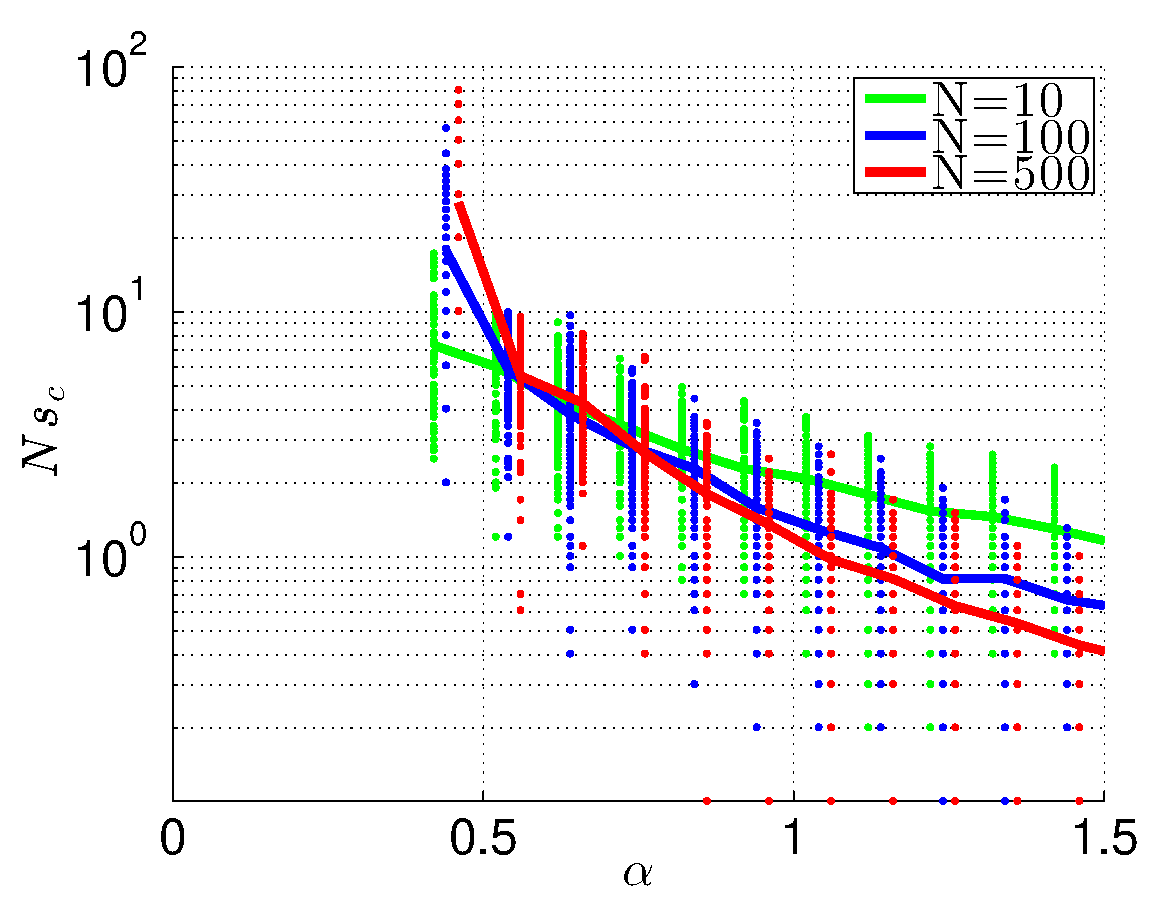
\includegraphics[height=3.5cm]{s_c_vs_alpha}


\emp


\Dn

\bmp{0.6\hsize}

{\bf Sparse disorder}

\Dn

Clean ring with  $M \ll N$ defects

$s_c \sim 1/N \ll s_1$

For $M$ field defects $s_c= \sigma \sqrt{M}/N$

\smp{0.4\hsize}

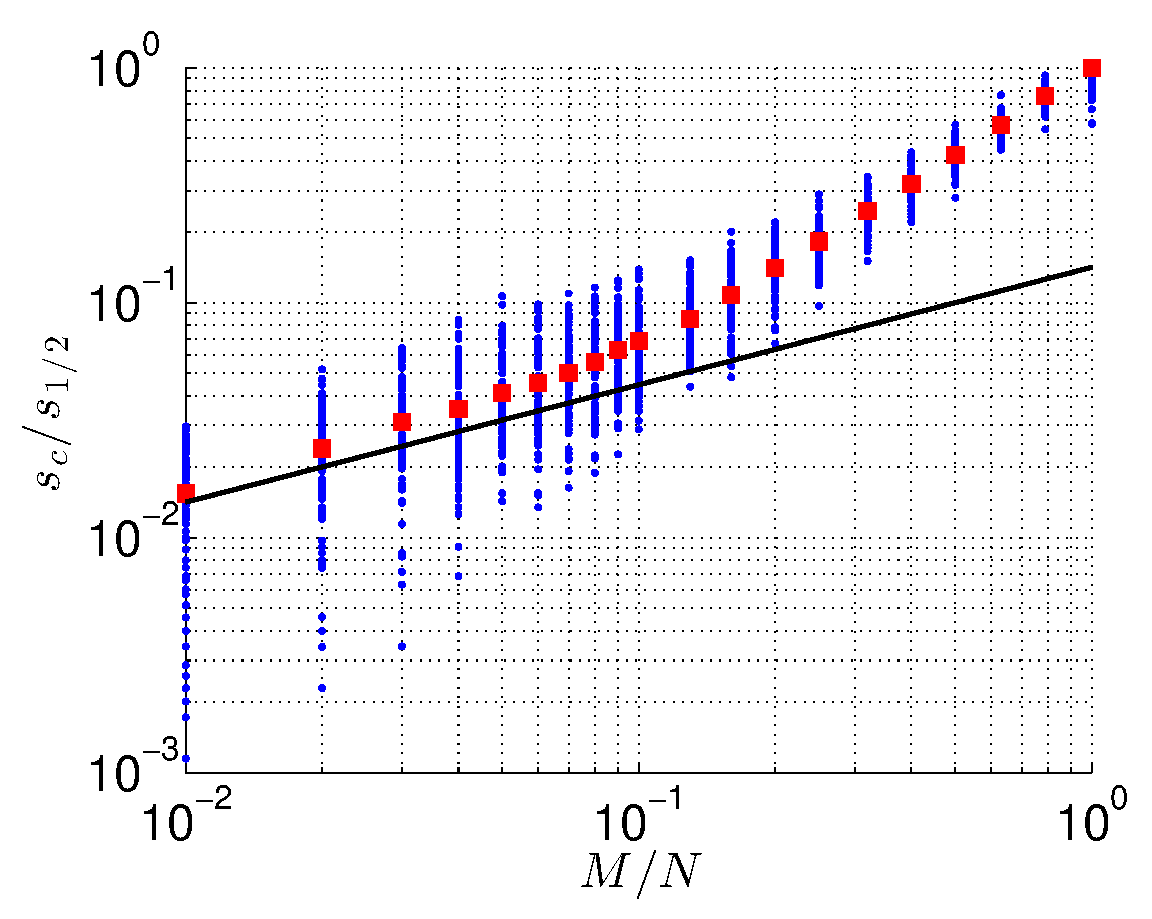
\includegraphics[height=3.5cm]{s_c_sparse_100_loglog}

\emp


\esl

\bslC

\Tl{\large Complexity saturation}

Recall the spectral determinant
%
$\displaystyle
\ \ \prod_{k=0}^{N-1} \left(\frac{z+\epsilon_k(s)}{\overline{w}}\right) \ \ = \ \ 2\left[\cosh\left(\frac{S_{\circlearrowleft}}{2}\right)-1\right]$


\bmp{0.6\hsize}

{\bf For large $s$ }

Non conservative $\leadsto$ entire spectrum becomes complex

Conservative $\leadsto$ complexity saturation

Trivial localization $\leadsto \epsilon_n = w_n \eexp{\mathcal{E}_n/2}$


\beq
\text{Upper cutoff $\epsilon_c$ determined by} \ \ \overline{\ln\left[ \epsilon - w\eexp{\mathcal{E}/2} \right]} \ \ = \ \ s/2 
\eeq

\smp{0.4\hsize}

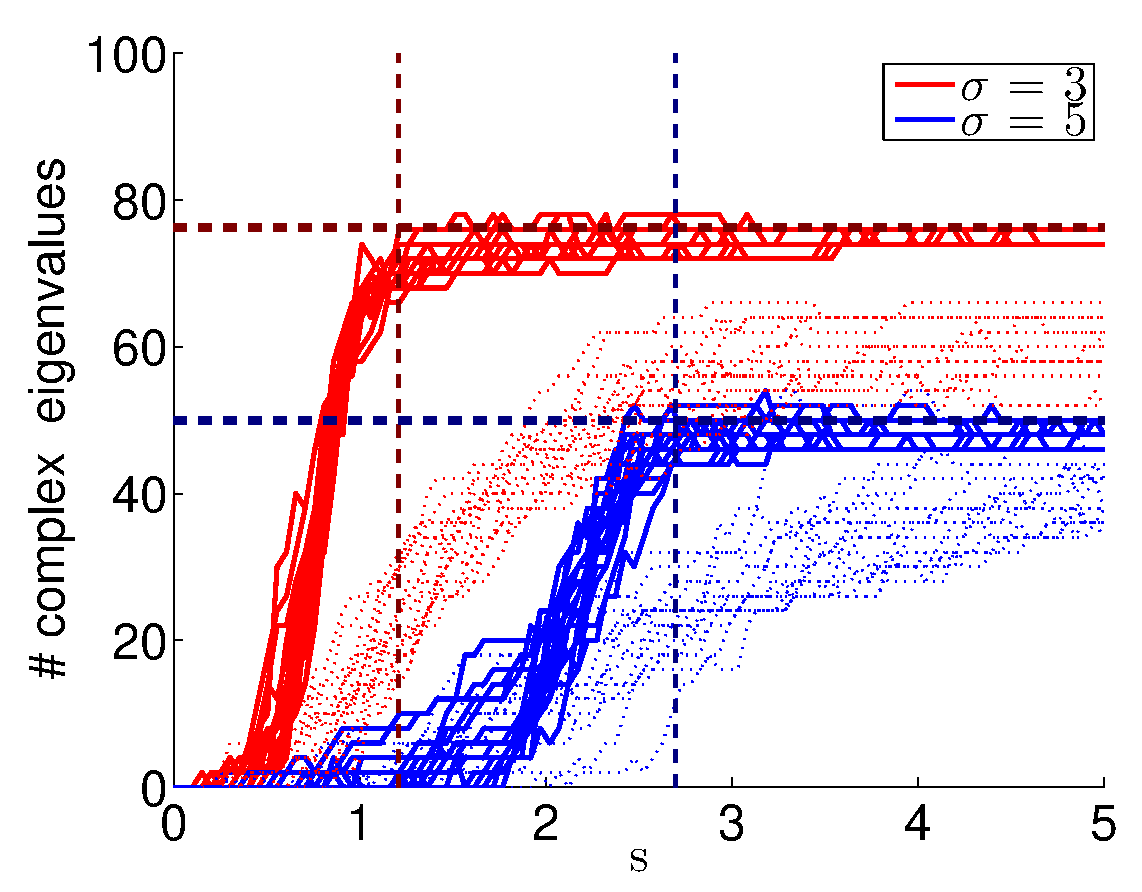
\includegraphics[height=3.5cm]{numComplex_100_alpha_sigma}

\emp

\esl

\end{document}


